\section{目标平台(Target)}

\textbf{1、RISC-V}

RISC-V是一个基于精简指令集(RISC)原则的开源指令集架构,其指令集设计简洁、高效,并且具有可扩展性。
与大多数指令集相比,RISC-V指令集可以自由地用于任何目的,允许任何人设计、制造和销售RISC-V芯片和软件而不必支付给任何公司专利费。
虽然这不是第一个开源指令集,但它具有重要意义,因为其设计使其适用于现代计算设备(如仓库规模云计算机、高端移动电话和微小嵌入式系统)。设计者考虑到了这些用途中的性能与功率效率。该指令集还具有众多支持的软件,这解决了新指令集通常的弱点。
RISC-V指令集的设计考虑了小型、快速、低功耗的现实情况来实做,但并没有对特定的微架构做过度的设计。

先前的比赛只有RISC-V一个主赛道,其中包括了k210,U740,和对应的QEMU模拟器三个平台。我们的NPUcore不仅支持了三个平台,同时也是k210榜单上唯一功能完整(能够通过所有性能测试项)的队伍,且U740平台上80\%性能测试项超越基准
而本次比赛还包括了LoongArch赛道,这也是我们国产自主的指令集架构,因此更具有里程碑式意义,因此我们果断选择参加了本赛道。

\textbf{2、 LoongArch}

2020年,龙芯中科基于二十年的CPU研制和生态建设积累推出了龙架构(LoongArch),包括基础架构部分和向量指令、虚拟化、二进制翻译等扩展部分,近2000条指令。

龙架构具有较好的自主性、先进性与兼容性。它从整个架构的顶层规划,到各部分的功能定义,再到细节上每条指令的编码、名称、含义,在架构上进行自主重新设计,具有充分的自主性。
龙架构摒弃了传统指令系统中部分不适应当前软硬件设计技术发展趋势的陈旧内容,吸纳了近年来指令系统设计领域诸多先进的技术发展成果。同原有兼容指令系统相比,不仅在硬件方面更易于高性能低功耗设计,而且在软件方面更易于编译优化和操作系统、虚拟机的开发。
龙架构在设计时充分考虑兼容生态需求,融合了各国际主流指令系统的主要功能特性,同时依托龙芯团队在二进制翻译方面十余年的技术积累创新,能够实现多种国际主流指令系统的高效二进制翻译。龙芯中科从 2020 年起新研的 CPU 均支持LoongArch。

今年的龙芯赛道,将基于2K1000开发板进行OSkernel开发。龙芯2K1000的结构如图\ref{fig:LA2K1000}所示。一级交叉开关连接两个处理器核、
两个二级Cache以及IO子网络(Cache访问路径)。二级交叉开关连接两个二级Cache、内存控制器、启动模块(SPI或者LIO)以及IO子网络(Uncache访问路径)。
IO子网络连接一级交叉开关,以减少处理器访问延迟。IO 子网络中包括需要 DMA 的模块(PCIE、GMAC、SATA、USB、HDA/I2S、NAND、SDIO、DC、GPU、VPU、CAMERA 和加解密模块)
和不需要DMA的模块,需要DMA的模块可以通过Cache或者Uncache方式访问内存。更详细的细节,可以参考龙芯官方提供的2K1000处理器用户手册。

\begin{figure}[htp]
    \centering
    \label{fig:LA2K1000}
    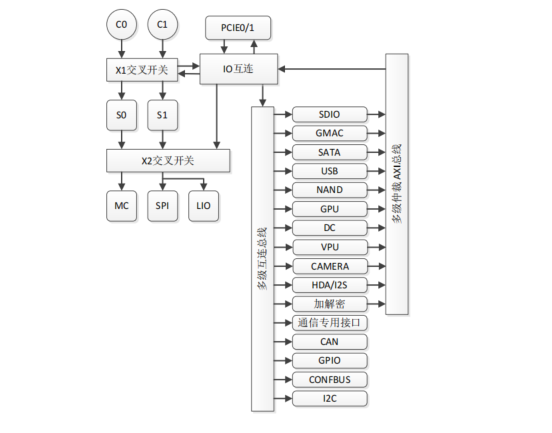
\includegraphics[width=0.7\linewidth]{figs/1-2.png}
    \caption{LA2K1000结构图}
\end{figure}

同时,大赛官方也提供了对应的Qemu版本\href{https://gitlab.educg.net/wangmingjian/os-contest-2024-image}{https://gitlab.educg.net/wangmingjian/os-contest-2024-image}(似乎有未解决bug)。
我们根据先前在RISC-V的经验,写了如下的runqemu脚本,则可以启动对应我们OS版本的2K1000-QEMU。
\begin{lstlisting}[language={bash},caption={uitl/qemu/runqemu}]
    #!/bin/bash
    DISK=/tmp/disk
    SCRIPTPATH="$( cd -- "$(dirname "$0")" >/dev/null 2>&1 ; pwd -P )"
    QEMU="$SCRIPTPATH"/bin/qemu-system-loongarch64
    [ -e $DISK ] || { truncate -s 32M $DISK;echo -e 'n\n\n\n\n\n\nw\nq\n'| fdisk /tmp/disk; }
    SUDO=$(if [ $(whoami) = "root" ];then echo -n "";else echo -n "sudo";fi)
    TFTP_DIR="$SCRIPTPATH"/../../easy-fs-fuse
    
    ls2k()
    {
    BIOS="$SCRIPTPATH"/2k1000/u-boot-with-spl.bin
    DEBUG_UNALIGN=1 DEBUG_GMAC_PHYAD=0 DEBUG_MYNAND=cs=0,id=0x2cda DEBUG_MYSPIFLASH=gd25q128 $QEMU \
        -M ls2k \
        -serial stdio \
        -drive if=pflash,file=$BIOS  \
        -m 1024 \
        -device usb-kbd,bus=usb-bus.0 -device usb-tablet,bus=usb-bus.0 \
        -device usb-storage,drive=udisk \
        -vnc :0 -D "$SCRIPTPATH"/qemu.log \
        -drive if=none,id=udisk,file=$DISK \
        -net nic -net user,net=192.168.1.2/24,tftp=$TFTP_DIR \
        -smp threads=1\
        -s -hda "$SCRIPTPATH"/2k1000/2kfs.img \
        -k "$SCRIPTPATH"/share/qemu/keymaps/en-us
    }
    
    ls2k "$@"
\end{lstlisting}
为了适配2K1000与龙芯架构,我们重构了大部分构建脚本,和底层硬件交互代码(约4000行)。这个过程非常曲折,遇到了各种各样繁复的问题,在这里我们已经没有办法一一说明了,这些细节我们都会在后续代码和注释中提到,希望可以对今后的队伍有所帮助。